\section*{Part 1}

I wrote the code based on the pseudocode for the algorithm on Geeks for Geeks \cite{astar_gfg}. 

\subsection*{Task 1}

\begin{figure*}[h!]
    \centering
    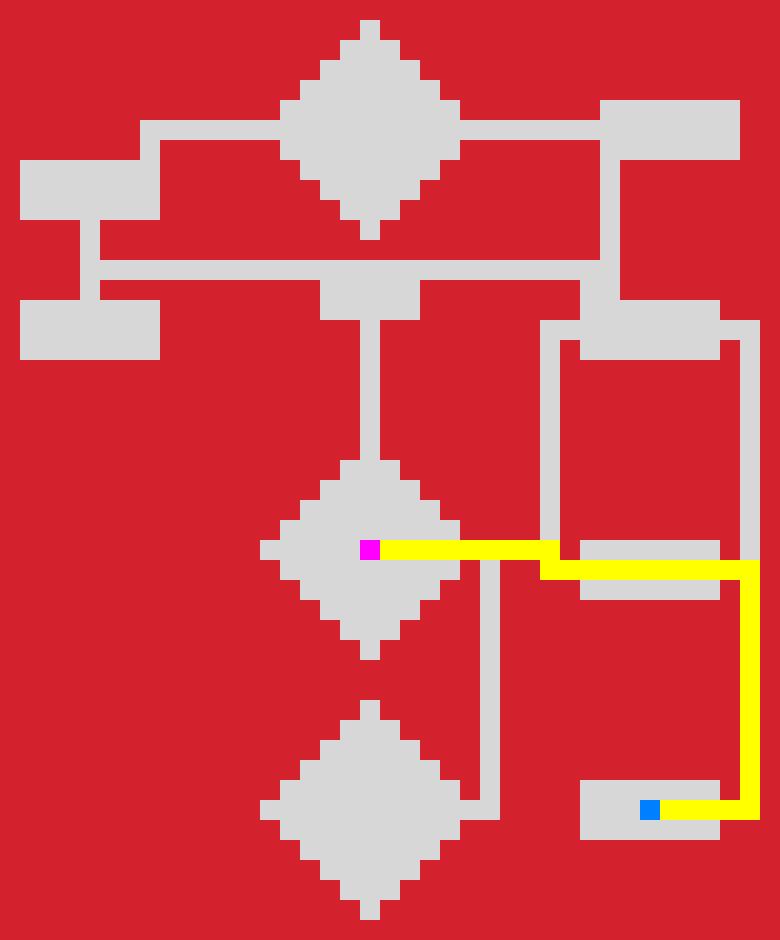
\includegraphics[width=0.4\textwidth]{"../Images/task_1.png"}
    \caption{Shortest path as found by the A* algorithm from the starting point (pink) to the goal (blue).}
\end{figure*}

\subsection*{Task 2}
\begin{figure*}[h!]
    \centering
    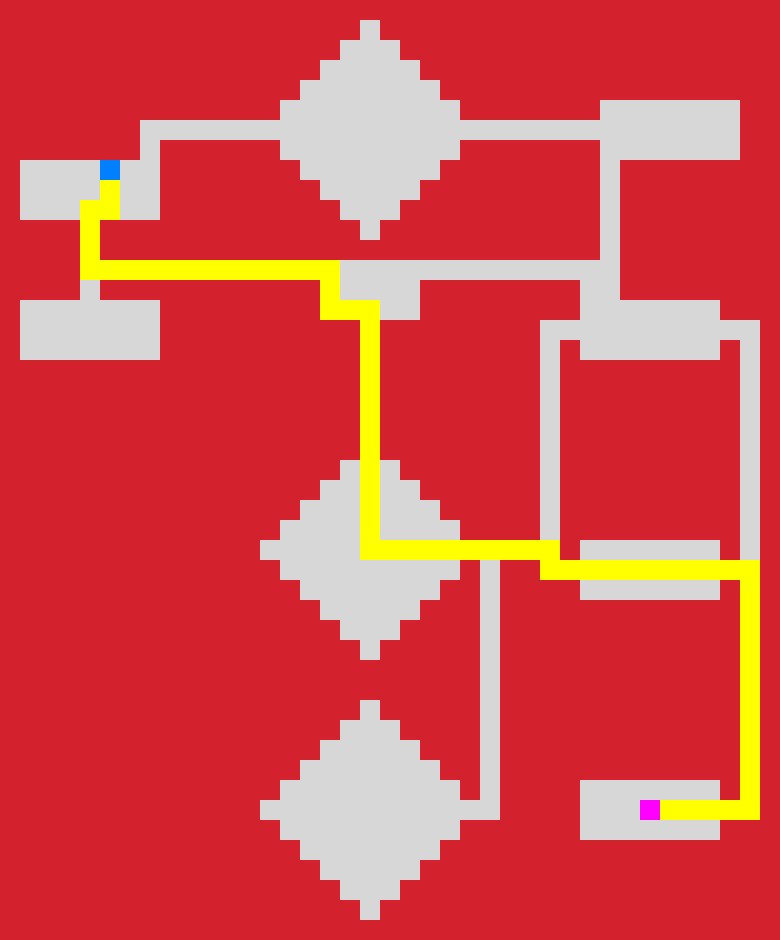
\includegraphics[width=0.4\textwidth]{"../Images/task_2.png"}
    \caption{Shortest path as found by the A* algorithm from the starting point (pink) to the goal (blue).}
\end{figure*}

\newpage

\section*{Part 2}

\subsection*{Task 3}
\begin{figure*}[h!]
    \centering
    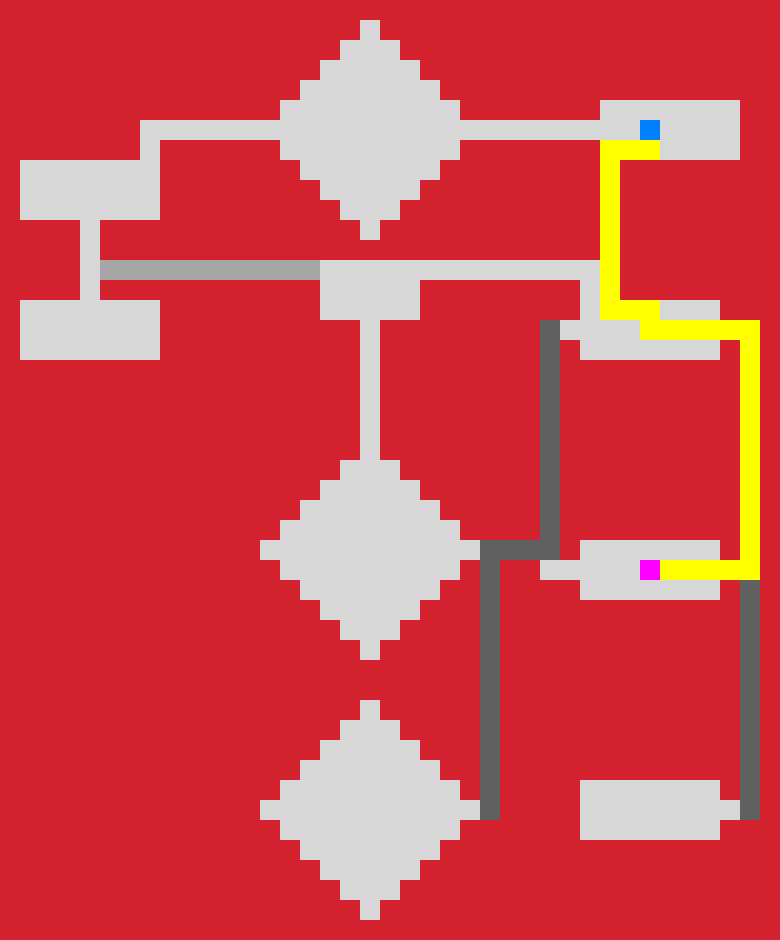
\includegraphics[width=0.4\textwidth]{"../Images/task_3.png"}
    \caption{Shortest path as found by the A* algorithm from the starting point (pink) to the goal (blue).}
\end{figure*}

\subsection*{Task 4}
\begin{figure*}[h!]
    \centering
    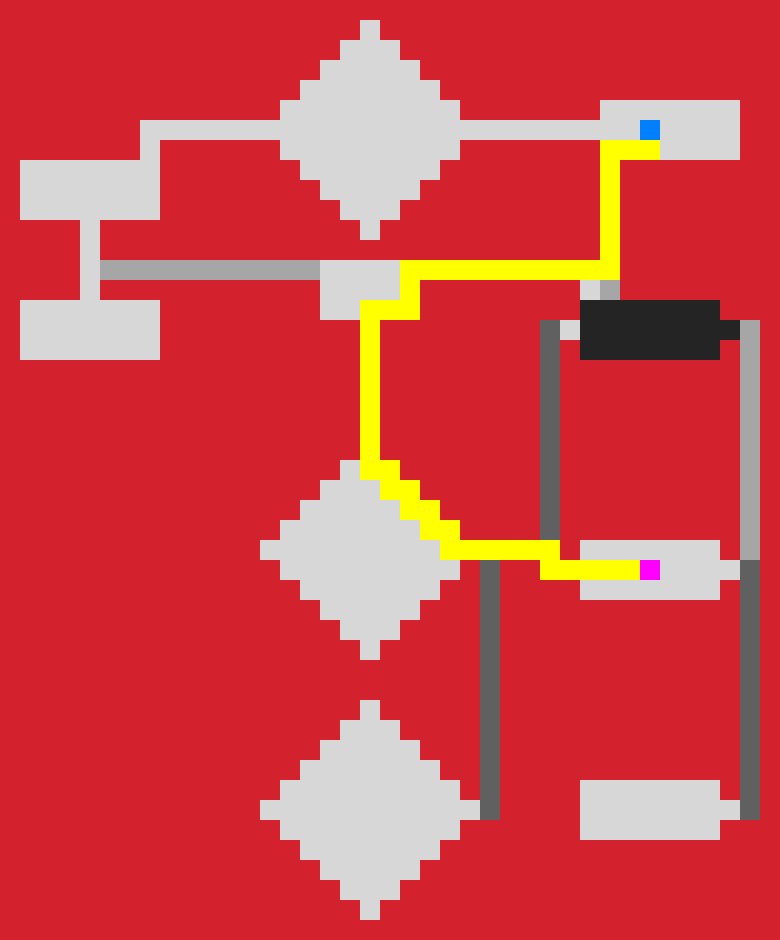
\includegraphics[width=0.4\textwidth]{"../Images/task_4.png"}
    \caption{Shortest path as found by the A* algorithm from the starting point (pink) to the goal (blue).}
\end{figure*}

\newpage

\section*{Part 3}

\subsection*{Task 5}
\begin{figure*}[h!]
    \centering
    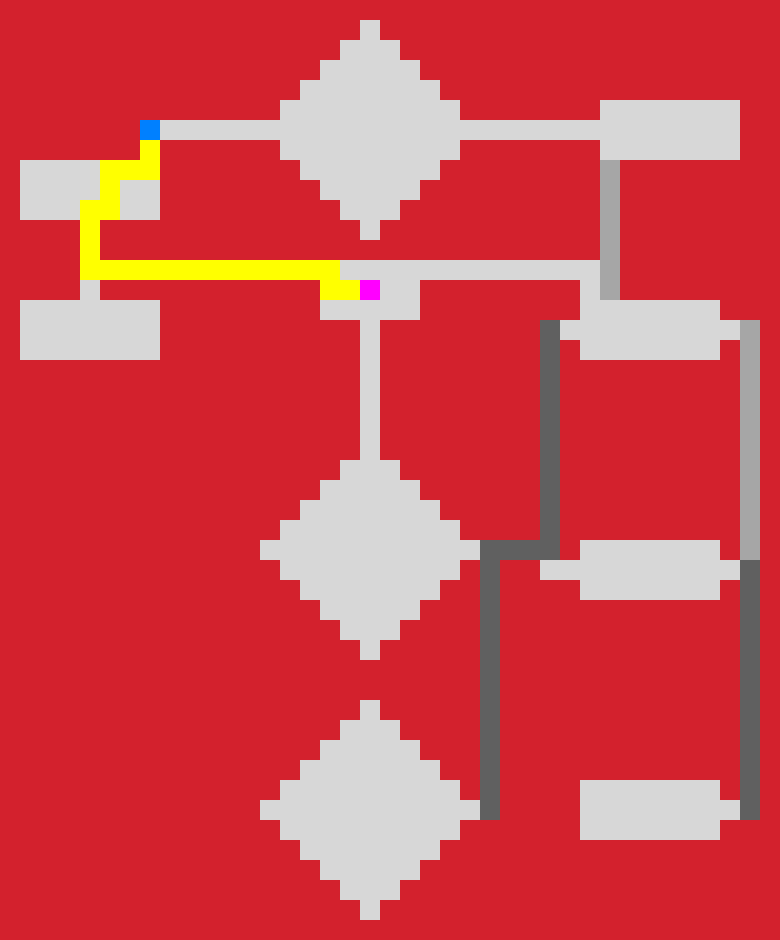
\includegraphics[width=0.4\textwidth]{"../Images/task_5.png"}
    \caption{Shortest path as found by the A* algorithm from the starting point (pink) to the moving goal (blue).}
\end{figure*}
